\section{Git：和远程仓库交互}

\begin{frame}{GitHub注册与配置}
    GitHub是目前最流行的Git仓库托管平台\footnote{\url{https://www.github.com}}，可以通过GitHub创建远程仓库。

    GitHub注册现在强制要求启用2FA认证，可以选择Microsoft Authenticator，具体来说，你需要在手机上安装这个应用，它会动态生成密钥，你在某些情况下需要输入这组密钥。推荐立即在Settings $\to$ General中将默认的主分支名由\code{main}改为\code{master}，避免不一致带来的麻烦。
\end{frame}

\begin{frame}{GitHub注册与配置}
    GitHub允许通过HTTPS和SSH两种方式与远程仓库交互，\alert{但你只应当使用SSH方式}，连接较为稳定，且免于在每次访问远程时输入密码。为此，你需要先在本地创建一对SSH密钥。

    SSH密钥采用RSA或ECC的加密算法\footnote{RSA基于大质数分解，ECC基于椭圆曲线。}，是一种非对称密钥。
    \begin{itemize}
        \item 密钥是成对的，一把是公钥，一把是私钥。
        \item 你应当将公钥提供给别人，而小心地保管私钥。
        \item 用于签名：使用你的私钥加密的数据，都只能用你的公钥解密。
        \item 用于加密：使用你的公钥加密的数据，都只能用你的私钥解密。
    \end{itemize}
\end{frame}

\begin{frame}{GitHub注册与配置}
    用以下命令生成SSH密钥。选项\code{-t rsa}代表使用RSA，选项\code{-b 4096}代表使用4096位的密钥，\code{-C "my-laptop"}代表密钥的注释，交互中，对每个问题直接按回车保持默认即可。
    
    这会生成公钥\code{\~/.ssh/id_rsa.pub}和私钥\code{\~/.ssh/id_rsa}两个文件。
    \begin{Code}*
        \lstinputlisting[firstline=1,lastline=1]{code/ssh-keygen.sh}
    \end{Code}
    查看公钥文件
    \begin{Code}*
        \lstinputlisting[firstline=2,lastline=2]{code/ssh-keygen.sh}
    \end{Code}
    复制显示的内容，在GitHub的Settings $\to$ SSH and GPG keys中点击New SSH Key，将复制的内容粘贴到Key中，将Title留空（Title会自动从密钥注释中被识别），随后点击确定就可以了。
\end{frame}

\begin{frame}{Git克隆远程仓库}
    你可以将远程仓库克隆到本地
    \begin{Code}*
        \lstinputlisting{code/git-clone.sh}
    \end{Code}
    部分Git仓库内会存在Git子模块，你需要在\code{git clone}时添加\code{--recursive}选项。
    
    如果在克隆时忘记加上这个选项，可以在克隆后执行以下命令拉取子模块。
    \begin{Code}*
        \lstinputlisting{code/git-submodule.sh}
    \end{Code}
\end{frame}

\begin{frame}{Git添加远程仓库}
    你需要首先在GitHub上手动创建一个远程仓库，为了后续使用的便利，\alert{不要让它自动生成任何文件}，包括\code{README}和\code{LICENSE}（这些可以在本地添加），确保这是一个干干净净的空仓库。

    添加一个远程仓库
    \begin{Code}*
        \lstinputlisting[firstline=1,lastline=1]{code/git-remote.sh}
    \end{Code}
    查看所有远程仓库
    \begin{Code}*
        \lstinputlisting[firstline=2,lastline=2]{code/git-remote.sh}
    \end{Code}
    远程仓库的名称可以是任意的，但\code{origin}是默认的远程仓库名称。
\end{frame}

\begin{frame}{Git添加远程仓库}
    删除一个远程仓库
    \begin{Code}*
        \lstinputlisting[firstline=3,lastline=3]{code/git-remote.sh}
    \end{Code}
    修改一个远程仓库的名称
    \begin{Code}*
        \lstinputlisting[firstline=4,lastline=4]{code/git-remote.sh}
    \end{Code}
    修改一个远程仓库的目标
    \begin{Code}*
        \lstinputlisting[firstline=5,lastline=5]{code/git-remote.sh}
    \end{Code}
\end{frame}

\begin{frame}{Git使用远程仓库}
    Git和远程仓库的交互主要有下面三条命令
    \begin{itemize}
        \item \code{git push}，将本地分支的提交，\alert{推送}到远程分支，用于上传（Push）。
        \item \code{git pull}，将远程分支的提交，\alert{拉取}到本地分支，用于下载（Pull）。
        \item \code{git fetch}，\alert{获取}远程分支的状态，用于刷新下载源（Fetch）。
    \end{itemize}
    总结：上传用\code{git push}命令，下载用\code{git pull}命令，刷新用\code{git fetch}命令！
\end{frame}

\begin{frame}{Git使用远程仓库}
    推送本地分支到远程
    \begin{Code}*
        \lstinputlisting[firstline=1,lastline=1]{code/git-push.sh}
    \end{Code}
    拉取远程分支到本地
    \begin{Code}*
        \lstinputlisting[firstline=1,lastline=1]{code/git-pull.sh}
    \end{Code}
    获取远程分支（但不更新本地分支）
    \begin{Code}*
        \lstinputlisting[firstline=1,lastline=1]{code/git-fetch.sh}
    \end{Code}
\end{frame}

\begin{frame}{Git使用远程仓库}
    当一个分支第一次向远程推送时，需要手动关联本地分支和远程分支
    \begin{Code}*
        \lstinputlisting[firstline=2,lastline=2]{code/git-push.sh}
    \end{Code}
    通过下面的配置，可以自动关联远程分支
    \begin{Code}*
        \lstinputlisting[firstline=3,lastline=3]{code/git-push.sh}
    \end{Code}
\end{frame}

\begin{frame}{Git使用远程仓库}
    实际上，\code{git pull}可以分解为\code{git fetch}和\code{git merge}两个步骤
    \begin{itemize}
        \item 第一步，\code{git fetch}的目的是刷新远程分支的本地副本\code{origin/master}。
        \item 第二步，\code{git merge}的目的是将\code{origin/master}合并到\code{master}。
    \end{itemize}
    如果远程分支和本地分支间发生了偏离，直接使用\code{git pull}命令将无法完成，其默认只允许快进。这时，你就需要通过\code{git fetch}命令和\code{git merge}命令手动拉取并合并远程分支。
    
    在实践中，请尽量避免这种情况！在多人合作中，每个人应当只在自己的分支上工作（例如命名为\code{liyx}和\code{lichf}）。由一个人负责定期合并到\code{master}分支，随后各自再同步\code{master}分支。
\end{frame}

\begin{frame}{关于Gradescope的使用提示}
    \begin{columns}
        \begin{column}{0.48\textwidth}\setlength{\parskip}{6pt}%
            \begin{itemize}
                \item 在GitHub上创建一个\alert{私有}仓库。
                \item 提交方式选择GitHub。
                \item Repository选择该次作业的仓库。
                \item Branch选择用于提交的分支。
            \end{itemize}
        \end{column}
        \begin{column}{0.48\textwidth}
            \begin{Figure}*
                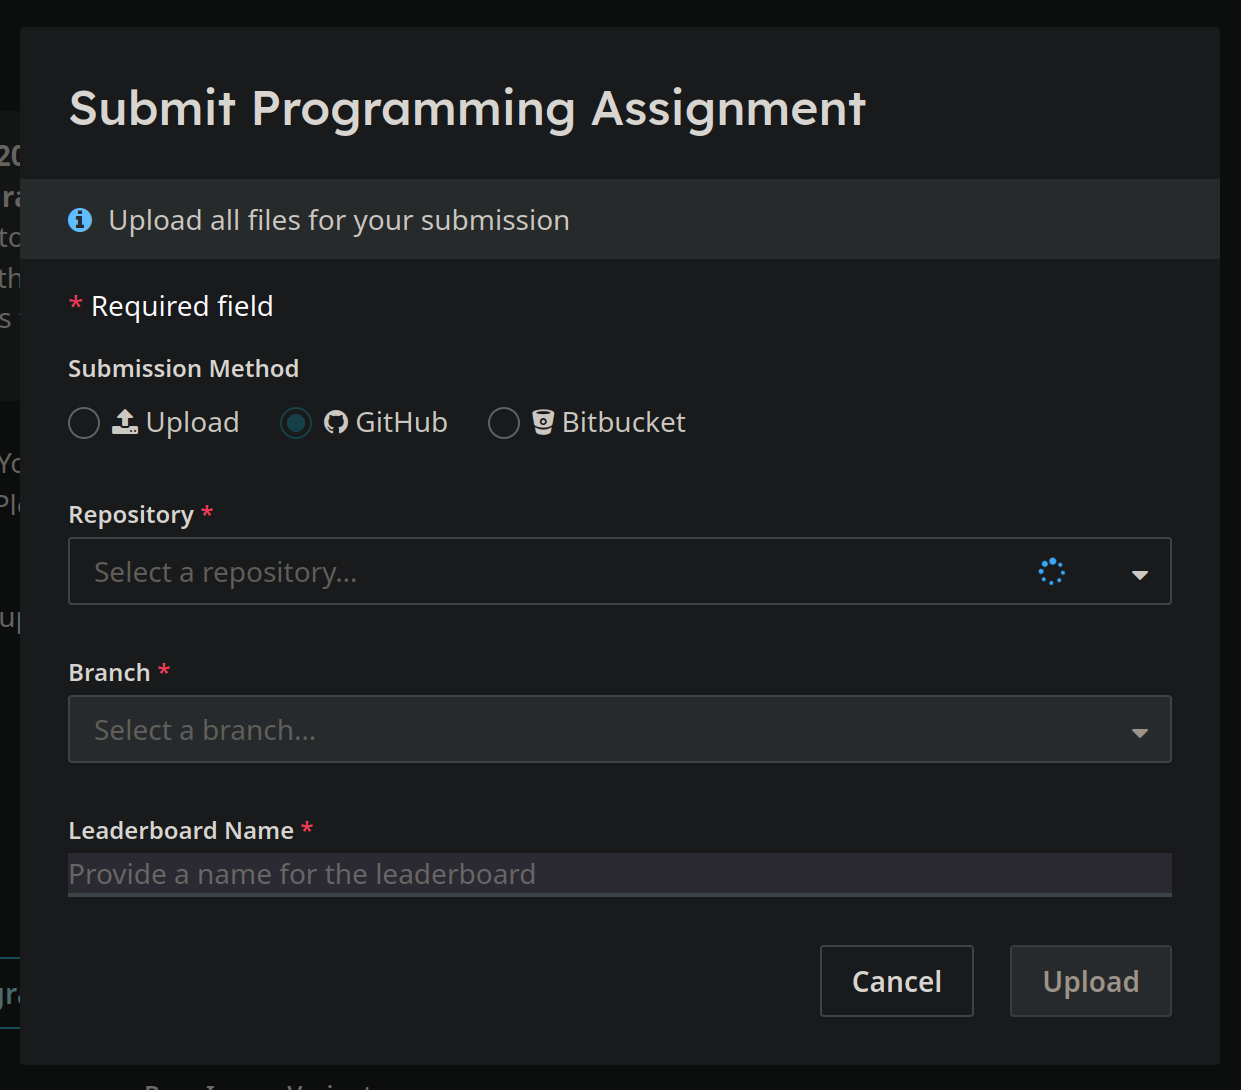
\includegraphics[width=\linewidth]{gradescope.png}
            \end{Figure}
        \end{column}
    \end{columns}
\end{frame}
